% Chapter 1

\chapter{Background Concepts} % Main chapter title

\label{Chapter2} % For referencing the chapter elsewhere, use \ref{Chapter1} 

\lhead{Chapter 2. \emph{Background Concepts}} % This is for the header on each page - perhaps a shortened title

%----------------------------------------------------------------------------------------
This chapter introduces the basic theory and mathematical concepts behind various Deep Learning model architectures. In particular, models and architectures which were or are State-of-the-Art in NLP have been discussed. 

\section{Neural Networks}

Research in the field of Machine Learning has been growing exponentially in the past decade. A majority of this progress can be attributed to a class of models - Deep Neural Networks(DNNs), commonly referred to as Neural Networks.

Neural Networks have been around for a long time, with early work on this subject appearing as early as the late 1950s in the form of the perceptron model\cite{Rosenblatt1958ThePA}. Another influential paper in this field is the 1986 paper, which introduced the backpropagation algorithm to update the weights of the network using partial derivatives\cite{Rumelhart1986LearningRB}. The methods described in this paper are still being used in modern-day Deep Learning.

While this worked well for shallower networks, it was very difficult to train deeper networks due to the computational limits of that time. Because of this, DNNs did not gain that much traction until the early 2010s, when growth of data and increased computational power, resulted in a boom in this field. 


\subsection{Neurons}

Neural Networks were developed to replicate the function of learning as a brain does. This is why their structure resembles connected neurons passing information, similar to how neurons fire in the human brain.

A neuron performs the same task as a mathematical function. It takes in a weighted sum of the inputs connected to it, adds a bias term and passes this sum through a non-linear function also called activation function. The equation is given below:

\begin{equation}
h = \underbrace{\sum_{i=1}^{\textit{k}} {W_i}{X_i}}_{\mathclap{\text{Weighted Sum of Input Neurons}}} +\smash{\overbrace{b}^{\mathclap{\text{Bias Term}}}}
\end{equation}

\begin{equation}
Y = \underbrace{\huge{\textit{f}}}_{\mathclap{\text{Non-Linear Activation}}} \, \bigl( h \bigr)  = \text{Neuron Output}
\end{equation}




\subsection{Structure}


\begin{figure}[htbp]
  \centering
    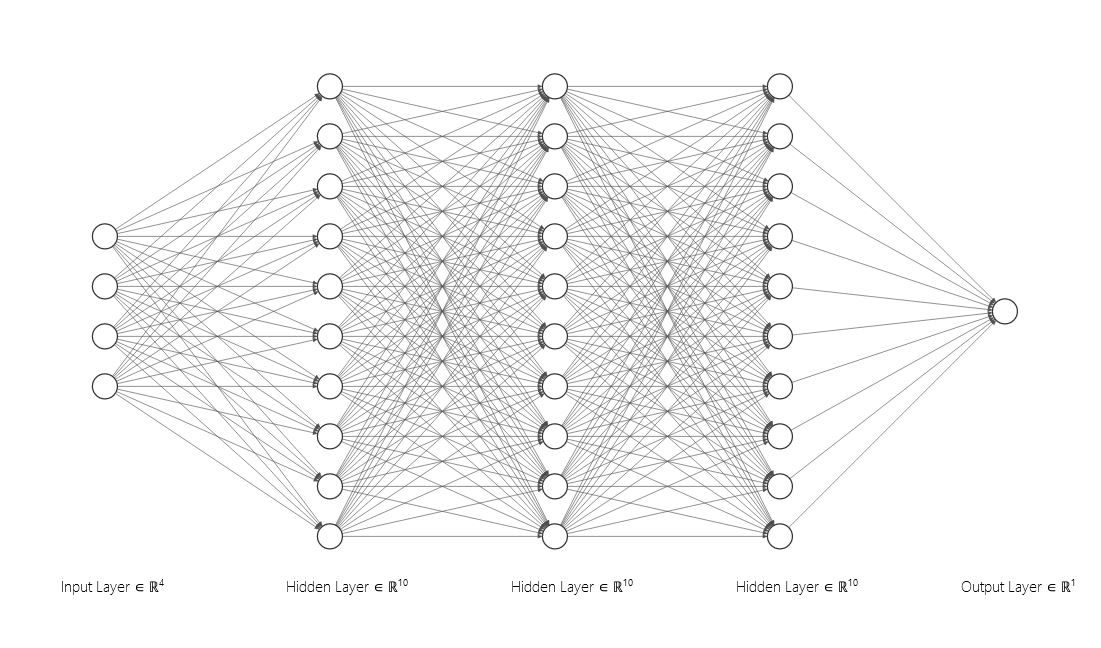
\includegraphics[scale=0.7]{Figures/nn_basic_fig.JPG}
    \rule{35em}{0.5pt}
  \caption[Vanilla Neural Network]{Basic Neural Network}
  \Source{https://alexlenail.me/NN-SVG/}
  \label{fig:basic_nn}
\end{figure}



\Sourc
\clearpage

DNNs consists of mainly three components:
\begin{itemize}[noitemsep,topsep=0pt]
    \item Input Layer
    \item \textit{n} number of Hidden Layers
    \item Output Layer
\end{itemize}

The input layer is the first layer in the network responsible for taking in the input. The information from this input layer gets passed on to the next hidden layer. This keeps on happening until the last hidden layer from which the information gets passed on to the output layer. At the output layer, the model output is used to calculate the loss, which is used to measure how far off the prediction of the network is as compared to the actual output. This loss then gets backpropagated through the neural network, updating the weights between the neurons. 

Other models discussed in the following chapters take inspiration from the architecture of Neural Networks and introduce changes resulting in models like RNNs and CNNs. These models perform well on specific data like Images or Text.


% Welcome to this \LaTeX{} Thesis Template, a beautiful and easy to use template for writing a thesis using the \LaTeX{} typesetting system.

% If you are writing a thesis (or will be in the future) and its subject is technical or mathematical (though it doesn't have to be), then creating it in \LaTeX{} is highly recommended as a way to make sure you can just get down to the essential writing without having to worry over formatting or wasting time arguing with your word processor.

% \LaTeX{} is easily able to professionally typeset documents that run to hundreds or thousands of pages long. With simple mark-up commands, it automatically sets out the table of contents, margins, page headers and footers and keeps the formatting consistent and beautiful. One of its main strengths is the way it can easily typeset mathematics, even \emph{heavy} mathematics. Even if those equations are the most horribly twisted and most difficult mathematical problems that can only be solved on a super-computer, you can at least count on \LaTeX{} to make them look stunning.

%----------------------------------------------------------------------------------------

\section{TF-IDF}

Term frequency – Inverse document frequency (TF-IDF) is a well known concept in Information Retrieval. Classifying documents, ranking web pages, and extracting relevant words from the corpus are some of the primary uses of TF-IDF. This method was introduced by Karen Spärck Jones in the 1972 article titled "A Statistical Interpretation of Term Specificity in Retrieval"\cite{kjones_tfidf}. 

Given a corpus with multiple documents, TF-IDF has two parts - Term Frequency(TF), which looks at how often a word appears in a specific document, and Inverse Document Frequency(IDF) which looks at how many times the word appears in different documents from the corpus. The reason is, words like "a" and "the" - which appear multiple times in text, won't be given much importance. But words that appear rarely will have a higher TF-IDF score. If a document contains the word "artificial" multiple times, but does not appear this often in other documents, then this document is relevant to searches related to the word "artificial". It will also have a high TF-IDF score for the particular word.

\clearpage
The formula to compute TF-IDF of words in a corpus of documents is as follows\cite{manning_raghavan_schütze_2008}:

\begin{equation}
    \resizebox{12.5cm}{!}
    {\displaystyle \mathrm {tf} (w,d)={\frac {f_{w,d}}{\sum _{w'\in d}{f_{w',d}}}} = \text{\small{Term Frequency for word \textit{w} in document \textit{d}}}}
\end{equation}
\begin{equation}
    \resizebox{14cm}{!}
    {\displaystyle \mathrm {idf} (w,D)=\log {\frac {N}{|\{d\in D:w\in d\}|}} = \text{\small{Inverse Document Frequency for word \textit{w} in corpus \textit{D}}}}
\end{equation}

where
\begin{fleqn}[1em]
\begin{flalign*}
{f_{w,d}} &= \text{Number of times $w$ appears in document $d$} \\
 {N} &= \text{Total Number of Documents in the corpus} \\
{\displaystyle{|\{d\in D:w\in d\}|}} &= \text{Number of documents where $w$ appears}
\end{flalign*}
\end{fleqn}
% \textit{N} = Total Number of Documents in the corpus, \\
% {\displaystyle{|\{d\in D:w\in d\}|}} = \text{Number of documents where \textit{w} appears}

Combining both these equations, we get the formula for calculating the TF-IDF score for a word \textit{w} in the corpus \textit{D}:
\begin{equation}
    {\displaystyle \mathrm {tfidf} (w,d,D)=\mathrm {tf} (w,d)\cdot \mathrm {idf} (w,D)}
\end{equation}

\section{CNN}

Convolutional Neural Networks(CNNs) are a class of neural networks that are used primarily for image recognition and classification. They were developed by Yann LeCunn in the 1990s for Optical Character Recognition(OCR) related tasks\cite{cnn_726791}.
\begin{figure}[htbp]
  \centering
    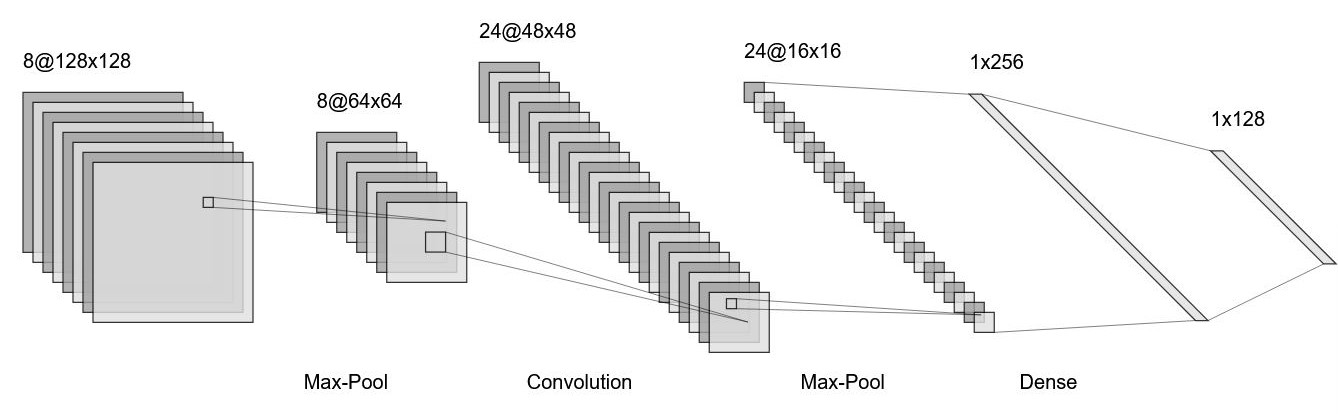
\includegraphics[scale=0.5]{Figures/cnn.JPG}
    \rule{35em}{0.5pt}
  \caption[Convolutional Neural Network]{CNN}
  \label{fig:cnn_architecture}
    \Source{https://alexlenail.me/NN-SVG/LeNet.html}
\end{figure}

Each layer in a CNN has filters which slide on the data from input/previous layer. Taking example of an grayscale image matrix as input to a CNN, the sliding window in this case would be a 2-D matrix of values which slides over the 2-D image detecting features like edges and lines. As we go towards the latter layers in a CNN, the features being detected go from edges and lines to ears and nose. 

\section{RNN}

Recurrent Neural Network(RNN) is a class of Neural Network which is primarily used for sequential data like Text, Audio and Time-Series data. Figure~\ref{fig:rnn_architecture} shows the architecture of an RNN cell.\\

\begin{figure}[htbp]
  \centering
    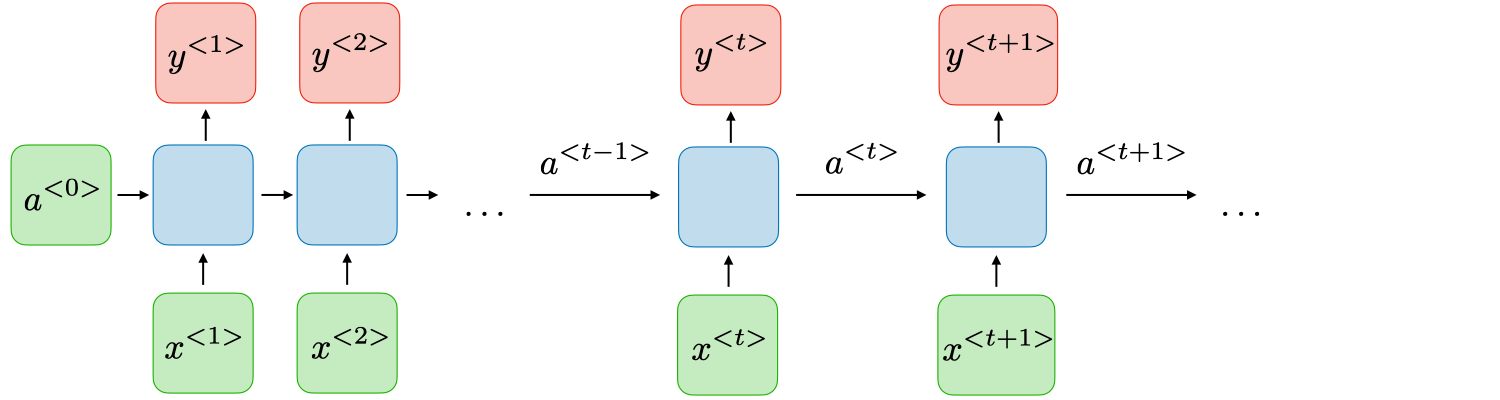
\includegraphics[scale=0.3]{Figures/architecture-rnn-ltr.png}
    \rule{35em}{0.5pt}
  \caption[Recurrent Neural Network]{RNN Architecture}
  \label{fig:rnn_architecture}
  \Source{https://stanford.edu/~shervine/teaching/cs-230/cheatsheet-recurrent-neural-networks}
\end{figure}

While neurons in a vanilla DNN can look at input data or data from the previous layer, the neurons in an RNN can go one step further. They can look at both - neurons from the last layer and the neuron output from the previous timestep. This small change in RNNs allows them to retain information from the past while calculating the output at a given timestep.

\begin{equation}
{
\resizebox{6.5cm}{!}{
\displaystyle 
{
    \begin{aligned}
    a^{<t>}&=
    {f}(W_{ax}x^{<t>}+W_{ay}y^{<t-1>}+b_{a})\\y^{<t>}&=
    {g}(W_{ya}a^{<t>}+b_{y})
    \end{aligned}}
}}
\end{equation}
where
\begin{fleqn}[1em]
\begin{flalign*}
f, g &= \text{Non-Linear Activation} \\
{x^{<t>}} &= t^{th} \text{ term of the input sequence} \\
{a^{<t>}} &= \text{Activation output at timestep = \textit{t}} \\
{y^{<t>}} &= \text{Neuron output at timestep = \textit{t}} \\
W_{ax},W_{ay}, W_{ya} &= \text{Weights} \\ 
b_{a}, b_{y} &= \text{Biases}
\end{flalign*}
\end{fleqn}

Based on the above equations, we can see how the output at a previous timestep, i.e. ${y^{<t-1>}}$, is used to calculate ${y^{<t>}}$. Theoretically, this means that past information will be used. But for practical use cases, this results in an issue known as Vanishing Gradient when performing a backward pass. To update weights in RNNs, Backpropagation through Time or BPTT is used. The derivation of the weight update rule in RNN shows that for input sequence length = \textit{N}, the derivative term contains weight raised to the power \textit{N}. This means that if the weight term is either very small or very large, the gradient will tend to zero or explode, respectively.

Architectures like LSTM and GRU addressed and corrected this shortcoming in RNNs.
\subsection{LSTM}

To avoid the problem of Vanishing Gradient, Schmidhuber and Sepp proposed a new kind of architecture\cite{lstm_schmidhuber} called Long-Short Term Memory (LSTM).Apart from the primary recurrence relation present in RNNs, LSTMs also have multiple gating mechanisms which allow it to choose the amount of information from the past that gets carried forward.

There are three different gates in an LSTM cell: 
\begin{itemize}[noitemsep,topsep=0pt]
    \item Forget Gate
    \item Input Gate
    \item Output Gate
\end{itemize}
The forget gate controls the amount of information that gets forgotten, the update gate controls the amount of information that gets carried forward, and the output gate controls the amount of information that gets passed on to the next layer.\\

\begin{figure}[htbp]
  \centering
    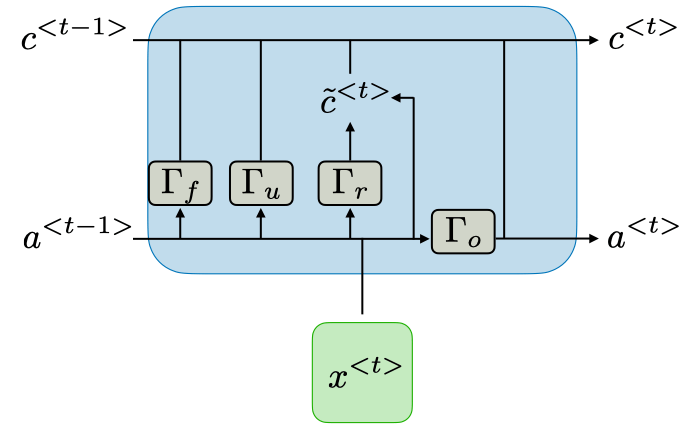
\includegraphics[scale=0.3]{Figures/lstm-ltr.png}
    \rule{35em}{0.5pt}
  \caption[LSTM]{LSTM Architecture}
  \label{fig:lstm_architecture}
    \Source{https://stanford.edu/~shervine/teaching/cs-230/cheatsheet-recurrent-neural-networks}
\end{figure}

The following equations show the working of an LSTM cell:

\begin{equation}
\begin{aligned}
&\Gamma_{r}=\tanh \left(W_{ca}a^{<t-1>} + W_{cx}x^{<t>} + +b_{c}\right)=\tilde{c}^{<t>} \\
&\Gamma_{u}=\sigma\left(W_{ua}a^{<t-1>} + W_{ux}x^{<t>} + +b_{u}\right) = \text{Update Gate}\\
&\Gamma_{f}=\sigma\left(W_{fa}a^{<t-1>} + W_{fx}x^{<t>} + +b_{f}\right) = \text{Forget Gate}\\
&\Gamma_{o}=\sigma\left(W_{oa}a^{<t-1>} + W_{ox}x^{<t>} + +b_{o}\right) = \text{Output Gate}\\
&c^{<t>}=\Gamma_{u} * \tilde{c}^{<t>}+\Gamma_{f} * c^{<t-1>} = \text{Memory Cell}\\
&a^{<t>}=\Gamma_{o} * \tanh \left(c^{<t>}\right) = \text{Activation Output}
\end{aligned}
\end{equation}
where
\begin{fleqn}[5.8em]
\begin{flalign*}
{\sigma}  &= \text{Sigmoid Function} \\
{*} &= \text{Hadamard Product (Element-Wise Multiplication)}
\end{flalign*}
\end{fleqn}

\subsection{GRU}

Gated Recurrent Units (GRUs) were proposed in 2014\cite{cho-etal-2014-learning}. They are similar to LSTMs but with a simpler architecture. Instead of the 3 gates that LSTM has, GRU only has 2 gates: Update Gate and Reset Gate.

This simplification in GRU makes it both, easier and faster to train compared to LSTM. The equations below show how information flows through a GRU cell at any given timestep: 

\begin{equation}
\begin{aligned}
&\Gamma_{r}=\sigma\left(W_{rx}x^{<t>} + W_{ra}a^{<t-1>} + b_{r}\right) = \text{Reset Gate} \\
&\Gamma_{u}=\sigma\left(W_{ux}x^{<t>} + W_{ua}a^{<t-1>} + b_{u}\right) = \text{Update Gate}\\
&\tilde{a}^{<t>}=\tanh \left(W_{ax}x^{<t>} + W_{ac}(\Gamma_{r}*a^{<t-1>}) + b_{c}\right) = \text{Candidate Activation}\\
&a^{<t>}=\Gamma_{u} * \tilde{a}^{<t>} + \left(1-\Gamma_{u}\right)* a^{<t-1>} = \text{Activation Output}
\end{aligned}
\end{equation}

\section{Transfomers}
\subsection{Attention Mechanism}
The Encoder-Decoder model worked well for machine translation tasks. The intuition behind the model was to use one RNN to encode and the other one to decode. The Encoder would encode the input sequence to generate meaningful embeddings and the other RNN - called the Decoder would use this embedding to generate translated output sequence.

But for purely RNN-based models, the model performance deteriorated with increasing input length.This changed with attention mechanism. In 2016, a paper titled "Neural Machine Translation by Jointly Learning to Align and Translate" \cite{Bahdanau2015NeuralMT} showed the power of attention for machine translation tasks. 
\begin{figure}[htbp]
  \centering
    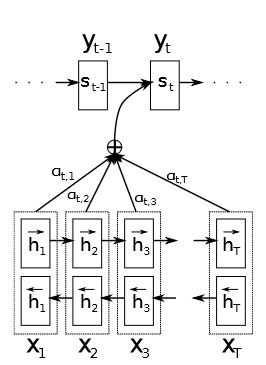
\includegraphics[scale=0.8]{Figures/bahdanau_attention_figure.JPG}
    \rule{35em}{0.5pt}
  \caption[Bahdanau Attention]{Bahdanau Attention}
  \label{fig:bahdanau_attention}
  \source{Figure 1 from "Neural Machine Translation by Jointly Learning to Align and Translate"\cite{Bahdanau2015NeuralMT}}
\end{figure}

The following equations show how context vector is calculated when decoding the output sequence: 
\begin{equation}
\begin{gathered}
\vspace{0.2cm}
e_{i j}=v_{a}^{\top} \tanh \left(W_{as} s_{i-1}+W_{ah} h_{j}\right)  = \text{Alignment Model} \\
\vspace{0.2cm}
\alpha_{i j}=\frac{\exp \left(e_{i j}\right)}{\sum_{k=1}^{T_{x}} \exp \left(e_{i k}\right)} = \text{Attention Weight} \\
c_{i}=\sum_{j=1}^{T_{x}} \alpha_{i j} h_{j} = \text{Context Vector}
\end{gathered}
\end{equation}
where
\begin{fleqn}[5.8em]
\begin{flalign*}
{h_j}  &= \text{$j^{th}$ Hidden state representation from Encoder} \\
{s_i} &= \text{$i^{th}$ Hidden state representation from Decoder}\\
{\alpha_{i j}} &= \text{Importance of $h_j$ when generating $s_i$ and $y_i$}
\end{flalign*}
\end{fleqn}

While there are other kinds of attention mechanisms\cite{luong-etal-2015-effective}, the one being used widely today is Multi-Head Self-Attention used in the Transformer architecture\cite{10.5555/3295222.3295349}. Self-Attention looks at each word in the input sequence and computes how important other words in the input are when computing the representation for that particular word. For this the input is first represented as a matrix of shape $(n,e)$ where $n = $ Length of Input and $e = $ Embedding dimension. 

From this input, we get three matrices : Key(K), Query(Q) and Value(V) by multiplying the input with weight matrices. The next equation shows how Self-Attention is computed using these matrices:

% Self attention
\begin{equation}
\text{Attention}(Q, K, V) = \text{softmax}\left(\dfrac{QK^T}{\sqrt{d_k}}\right)V 
\end{equation}

The dot product between $Q$ and $K^T$ computes the similarity between the current word and all the other words in the input sequence.$\sqrt{d_k}$ (dimension of Key matrix) is used to scale down the dot product so that the gradient does not become unstable for large values of $n$. Softmax converts this to a probability distribution which adds up to 1. The final multiplication with Value matrix results in those words retaining their embedding whose dot-product score is high, which results in meaningful and contextual embeddings. 

This shows the working of a single Self-Attention head. Transformers have multiple such heads, the outputs of which are concatenated and transformed into a compatible dimension. Another feature of transformer models is that they use multiple encoders and decoders stacked on top of each other as their Encoder and Decoder blocks. 
Figure~\ref{fig:vaswani_transformer} shows the model architecture of a Transformer as provided by the authors in the original paper.
\begin{figure}[htbp]
  \centering
    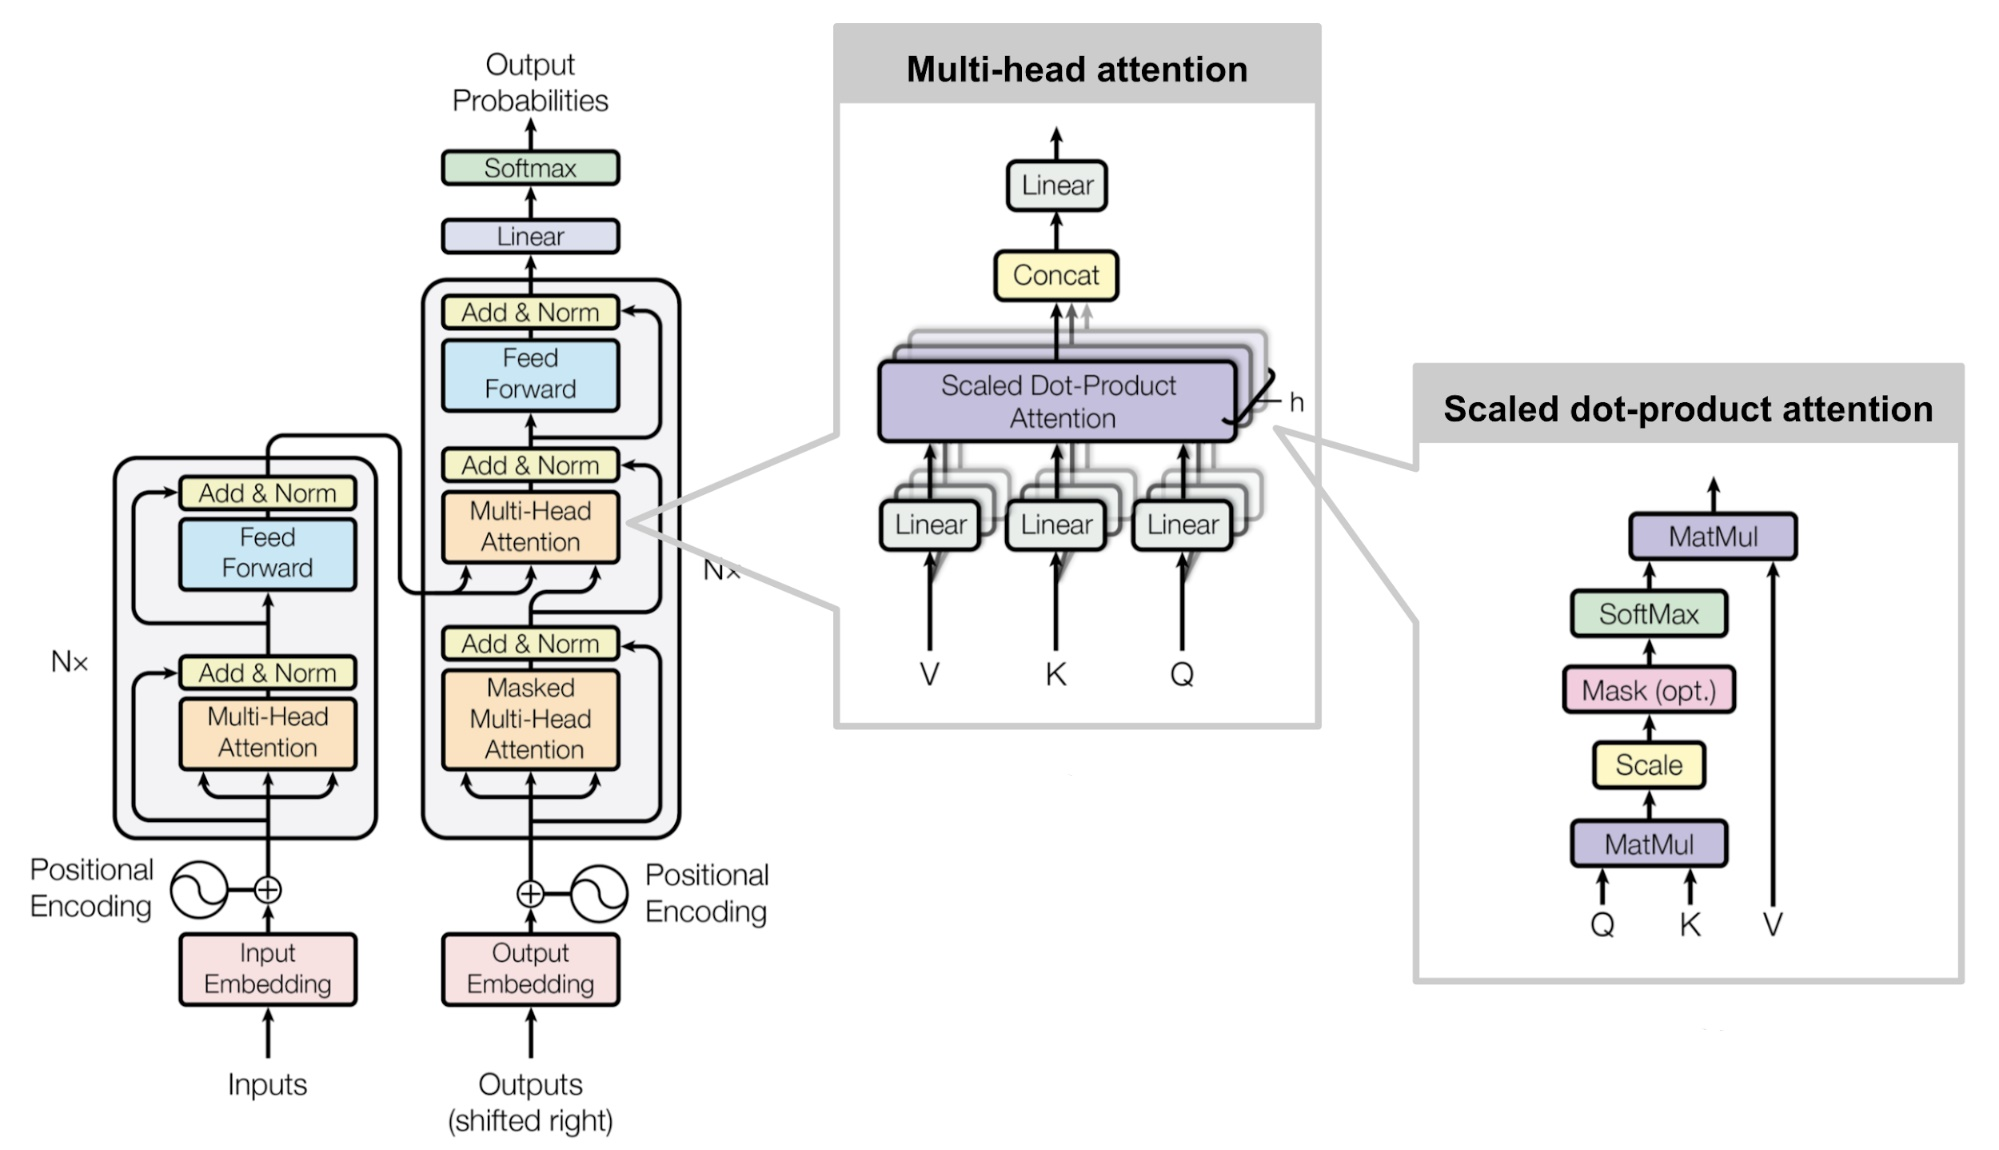
\includegraphics[scale=0.18]{Figures/vaswani_transformer.jpg}
    \rule{35em}{0.5pt}
  \caption[Transformer Architecture]{Transformer Architecture}
  \label{fig:vaswani_transformer}
  \Source{https://lilianweng.github.io/lil-log/2018/06/24/attention-attention.html}
\end{figure}

\clearpage
\subsection{BERT}

Bidirectional Encoder Representations from Transformers (BERT) was originally published by Google AI Language in 2018 where they used the transformer architecture for the task of language modeling\cite{devlin-etal-2019-bert}. One of the key features of BERT is that it stacks only Encoder blocks on top of each other.

BERT is deeply bidirectional i.e. the model learns from both left-to-right and right-to-left while going over input sentences. Also the self-attention combined with multi-head attention in each transformer encoder block helps to generate more contextual embeddings by taking into account other words in the sentence when encoding a particular word. Multiple attention heads, deep bidirectional nature coupled with the combined training task of Masked Language Modelling and Next Sentence Prediction are some of the reasons why the BERT language model has a really good understanding of the structure and semantics of English language. Due to these reasons, a single dense layer on top of the output of the BERT language model performs exceptionally well on many NLP tasks.


\subsection{RoBERTa}

Robustly Optimized BERT Pretraining Approach (RoBERTa) is an alternate approach to training BERT which not only improves it performance but also results in easier training\cite{liu2019roberta}.

BERT masks token randomly during preprocessing stage resulting in a static mask. And to avoid using the same masked sequence every epoch, the training data for BERT was duplicated multiple times so that each sequence can be masked in multiple ways. But this becomes difficult to implement with large datasets.To addresss this, authors of RoBERTa propose a dynamic masking scheme which means that masking takes place before a sentence gets selected into a minibatch to be fed into the model.